\documentclass[11pt, a4paper]{article}
\usepackage[nochapters]{classicthesis}                              % template
\usepackage[margin=42mm]{geometry}                                  % margins
\usepackage[utf8]{inputenc}                                         % allow utf-8 input
\usepackage[T1]{fontenc}                                            % use 8-bit T1 fonts
\usepackage{graphicx}                                               % images
\usepackage{url}                                                    % URL typesetting
\usepackage{booktabs}                                               % good-looking tables
\usepackage{multirow}                                               % for tables
\usepackage{amsfonts}                                               % blackboard math symbols
\usepackage{amsmath}                                                % math ops
\usepackage{nicefrac}                                               % compact 1/2, etc.
\usepackage{microtype}                                              % microtypography

\definecolor{darkblue}{rgb}{0, 0, 0.5}                              % define link color
\hypersetup{colorlinks=true,citecolor=darkblue,                     % set link color
            linkcolor=darkblue, urlcolor=darkblue}

% Your packages here
% \usepackage{...}                                                  % some info, maybe

% !!! PLEASE CHANGE THESE VARIABLES TO MATCH YOUR INFORMATION !!!

\def\thesistitle{Multi-class Alzheimer's Disease classification from structural MRI using Vision Transformers}                      % title
\def\subtitle{A comparison of data-efficient and hierarchical Vision Transformers}             % subtitle
    % ^if there is no subtitle, replace by \def\subtitle{}  
\def\yourname{M.D.W. van der Wielen}                                                                       % ^first and last name
\def\yourprogramme{Data Science \& Society}                         % OR (remove this)
% \def\yourprogramme{Cognitive Science \& Artificial Intelligence}    % uncomment this
\def\yourstudentnumber{2027613}                                      % ANR (or u-number)
\def\finalmonth{January}
\def\finalyear{2000}
\def\supervisor{dr. J. S. Olier Jauregui}
\def\committee{dr. G. Saygili}
\def\acknowledgments{Some room for acknowledgements.}

% METADATA

\hypersetup{pdfauthor   = \yourname,
            pdftitle    = \thesistitle\ \subtitle,
            pdfsubject  = \yourprogramme\ Master Thesis
}

% CHOOSE EITHER OF -----------------------------------------
% IEEE STYLE:

% \usepackage[square,numbers]{natbib}                               % bracket-style refs
% \usepackage{natbib}                                               % OR: parenthesized refs
% \bibliographystyle{IEEEtranN}

% OR -------------------

\usepackage[natbibapa]{apacite}                                     % only parentheses
\bibliographystyle{apacite}                                         % 'cause APA

% !!! ------------------------------------------------------ !!!

\begin{document}
% DON'T TOUCH THIS FILE, THANKS!

\pagenumbering{gobble}
\thispagestyle{empty}

\newgeometry{margin=30mm}
\begin{center}
\hspace{0.75cm}
\includegraphics[scale=0.5]{logo.eps} \\
\vspace{5cm}
\huge\spacedallcaps{\thesistitle} \\ [0.5cm]
\Large\spacedallcaps{\subtitle} \\ [1.2cm]
\normalsize\spacedallcaps{\yourname{}} \\ [1cm]
\normalsize{\spacedlowsmallcaps{Thesis submitted in partial fulfillment}} \\
\normalsize{\spacedlowsmallcaps{of the requirements for the degree of}} \\
\normalsize{\spacedlowsmallcaps{Master of Science in \yourprogramme{}}}\\
\normalsize{\spacedlowsmallcaps{at the School of Humanities and Digital Sciences}} \\
\normalsize{\spacedlowsmallcaps{of Tilburg University}} \\ [5cm]
\normalsize{\spacedlowsmallcaps{Word count: ...}} \\
\end{center}
\restoregeometry

\newpage

\begin{tabular}{l}
\noindent \spacedlowsmallcaps{student number} \\ [0.2cm]
\yourstudentnumber \\ [0.5cm]
\spacedlowsmallcaps{Committee} \\ [0.2cm]
\supervisor \\
\committee\\ [0.5cm]
\spacedlowsmallcaps{location} \\ [0.2cm]
Tilburg University    \\                        
School of Humanities and Digital Sciences \\
Department of Cognitive Science \& \\
Artificial Intelligence \\
Tilburg, The Netherlands \\ [0.5cm]
\spacedlowsmallcaps{date} \\ [0.2cm]
\today \\
\end{tabular}
\vfill
\begin{tabular}{p{12cm}}
\spacedlowsmallcaps{acknowledgments} \\ [0.2cm]
%\noindent \acknowledgments{}
Firstly, I want to thank J. S. Olier Jauregui for his useful feedback and insights throughout the writing of this thesis. His guidance helped me write a thesis that aligned with the goals that I set at the start of the period. Secondly, I want to thank G. Saygili and E. Postma for the useful discussions and feedback that ultimately shaped my thesis. Finally, I want to thank my family, friends and girlfriend for supporting me during this period.
\end{tabular}

\newpage \pagenumbering{arabic}

\title{\rmfamily\normalfont\spacedallcaps{\thesistitle}\\[0.2cm]
       \rmfamily\small\spacedallcaps{\subtitle}}
\author{\spacedlowsmallcaps{\yourname}}
\date{}

\maketitle  % don't remove this :)

% --- start writing below:

\begin{abstract}
The currently ongoing negative trends concerning Alzheimer’s Disease (AD) call for improved methods for early AD detection. Mild Cognitive Impairment (MCI) is the prodromal stage of AD. Detecting MCI early could give room for opportunities to slow down or completely prevent the conversion to AD. For a long time, 2D and 3D convolutional neural networks (CNN) have been superior in classifying AD stages. The relatively new Vision Transformer (ViT) shows promising results in all computer vision domains. However, the need for large-scale datasets and high computational power limits their applicability in the medical image classification domain. Therefore, the Data-efficient image Transformer (DeiT) and Swin Transformer are investigated in this research. The DeiT is better able to deal with small-scale datasets. The linear computational complexity of the hierarchical Swin Transformer makes it more computationally efficient compared to other ViTs. The ViT models are compared against VGG16, a state-of-the-art 2D CNN. The models were trained on a pre-processed AD dataset from the Kaggle website, after which they were evaluated on accuracy, precision, recall, the F1-score, and training time. The VGG16 beats the DeiT and Swin on accuracy by 4.2\% and 5.8\% respectively, achieving an accuracy of 91.9\%. An arguably more important metric for this research is the recall of the ‘mild demented’ class. For this class, the DeiT and Swin achieve a recall of 68.9\% and 66.7\% respectively. The VGG16 outperforms them with a substantially higher recall of 83.0\%. Therefore, it can be concluded that 2D CNNs remain the best-performing models for AD classification, and more research is necessary to unlock the full potential of ViTs.
\end{abstract}
\newpage
\section{Data source / code / ethics statement}
Work on this thesis did not involve collecting data from human participants or animals. The publicly available Alzheimer’s Disease dataset was obtained from the Kaggle website through \href{https://www.kaggle.com/datasets/tourist55/alzheimers-dataset-4-class-of-images}{\textbf{this}} link. The MRI images in the dataset are anonymized. The original owner of the data used in this thesis retains ownership of the data during and after the completion of this thesis. The author of this thesis acknowledges that they do not have any legal claim to this data. All figures and tables used in this thesis were produced by the author. The code used in this thesis is publicly available on GitHub \href{https://www.kaggle.com/datasets/tourist55/alzheimers-dataset-4-class-of-images}{\textbf{here}}. 

\section{Introduction} \label{sec:introduction}
Alzheimer’s Disease (AD) is a progressive neurological disorder where the degeneration of nerve cells in the brain causes memory loss, decreased cognitive abilities, and personality change. It can eventually lead to death caused by complete brain failure \citep{BrightFocusFoundation2022Alzheimers:Stats}. At first, it was thought that the brain changes occur due to an accumulation of abnormal proteins and phosphorylated tau in the brain \citep{20222022Figures}. However, a recent study indicates that it may also be caused by an absence of hard cognitive demand \citep{Turknett2022DemandDementia}.

Here you write the introduction. You can refer to chapters like the current Section~\ref{sec:introduction}. If you want to list research questions it's probably best to use \texttt{quote} and/or \texttt{itemize}, like so:

\begin{quote}
\emph{To what extent we define a main research question?}
\end{quote}



\noindent The sub-questions can be listed seperately, as such:

\begin{itemize}
    \item[RQ1] \emph{How does sub question one influence the main RQ?}
    \item[RQ2] \emph{To what degree does sub question add anything?}
\end{itemize}

\noindent Or, format it as you desire (tip: you can nest \texttt{itemize} as well). You can alternate \emph{emph} and \textbf{textbf} however you wish. This should cover most of the things required for the introduction.

\section{Related Work}


Copy paste BibTeX code\footnote{Using e.g. the quote icon in GScholar, then BibTeX at the bottom.} and put it in \texttt{references.bib}. After, you can cite some work \citep{mackay2003information} -- using \texttt{\textbackslash citep}. You can refer to the author of e.g. \cite{minsky1961steps} directly like using \texttt{\textbackslash cite} (this does not work when using bracket-citation). If you use bracket-style,\footnote{Find the \texttt{natbib} part in the \texttt{main.tex} \LaTeX{} script.} you might want use \texttt{\textbackslash citeauthor} when citing, like: see \citeauthor{ananny2018seeing} \cite{ananny2018seeing}.  If you want to add pages you can use brackets in \texttt{\textbackslash citep[][p. 5]\{mackay2003information\}}, which looks like: \citep[][p. 5]{mackay2003information}. The first brackets can be used for things like \emph{see}, and \emph{e.g.}. If you want to cite multiple authors, simply comma-separate them (\texttt{\textbackslash citep\{\-minsky\-1961\-steps,\-mackay\-2003\-information\}}) and it will aggregate them automatically \citep{minsky1961steps,mackay2003information}.

\section{Method}

If you define any equations (\verb|\begin{equation}...|), you probably might want to define everything using math operators (e.g., \verb|$D$|) and cite the work (!). So for example, following \cite{lewis1994sequential}, representing a document $d \in D$ as tf$(d)$, we define a probabilistic model $(d | Y = y)$ for all documents in class $y$, and select $y$ most likely to generate $d$:

\begin{equation} \label{eq:nbarg}
    \hat{y} = \underset{y}{\mathrm{argmax}} \ P(d | y) \cdot P(y)
\end{equation}

With this we can detect spam (see Figure~\ref{fig:spam}) or bots.  Note that the figures (and tables for that matter) might not always be placed in this section (oh no)! \LaTeX{} determines where to best put your objects, so don't worry about that. The reader will find them. \textbf{NOTE}: this Figure has a Creative Commons license; you cannot re-use other authors' figures without explicit permission or permissive licensing (as this would mean copyright infringement). You can refer to the equations as well (Equation~\ref{eq:nbarg})!

\begin{figure}
    \centering
    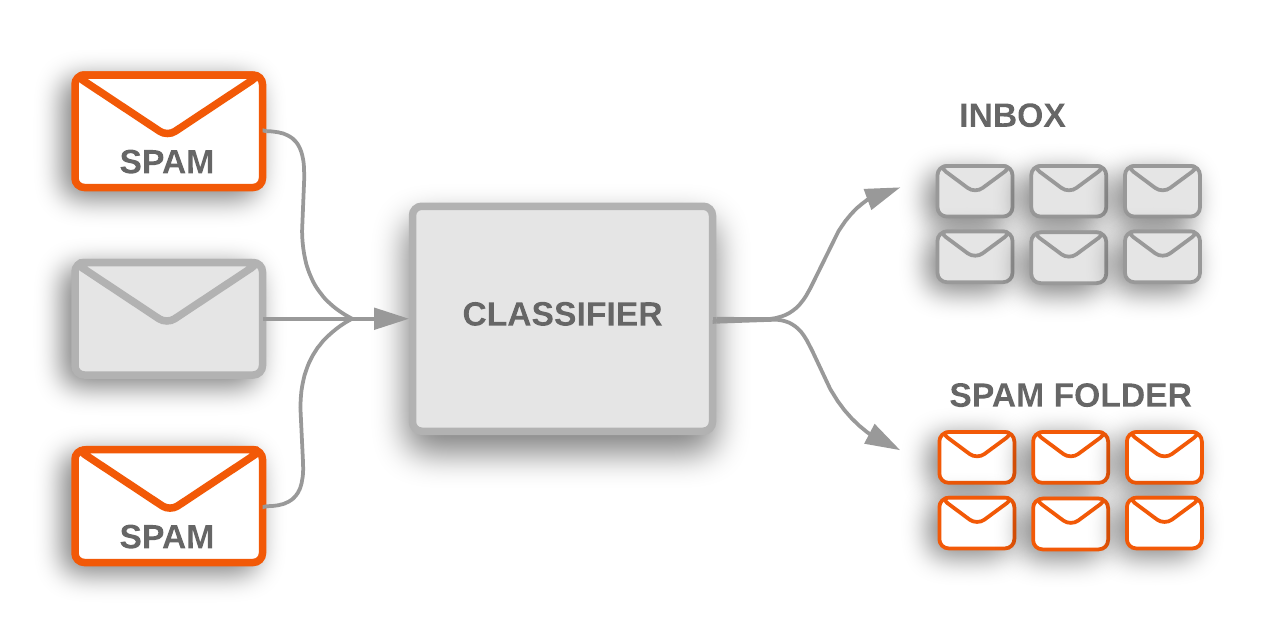
\includegraphics[width=\textwidth]{spam.png}
    \caption{Spam classification example. Source: \href{https://developers.google.com/machine-learning/guides/text-classification}{Google} (CC BY 4.0).}
    \label{fig:spam}
\end{figure}

\section{Results}

\begin{table}[]
    
\begin{tabular}{@{}lrrrrl@{}}
\toprule
\textbf{Model} & \multicolumn{1}{l}{\textbf{Accuracy}} & \multicolumn{1}{l}{\textbf{Precision}} & \multicolumn{1}{l}{\textbf{Recall}} & \multicolumn{1}{l}{\textbf{F1-score}} & \textbf{Computation time} \\ \midrule
VGG16          & \textbf{0.9185}                       & \textbf{0.8888}                        & \textbf{0.8942}                     & \textbf{0.8914}                       & \textbf{18 minutes}       \\
DeiT-B         & 0.8770                                & 0.7688                                 & 0.8720                              & 0.8075                                & 42 minutes                \\
Swin-B         & 0.8610                                & 0.7078                                 & 0.8005                              & 0.7411                                & 37 minutes                \\ \bottomrule

\end{tabular}
    \caption{Performance metrics for the VGG16, DeiT-B and Swin-B model. The precision, recall and F1-score are macro averages.}
\end{table}

\begin{table}
    \caption{Best scoring models classifying bots, on Twitter and Facebook respectively. $F_1$ scores report positive (bot) class. Outline text left (l) and numbers right (r).}
    \label{tab:results}
    \centering
    \small
    \begin{tabular}{llrr}
        \toprule
                              &                                   & \multicolumn{2}{c}{$F_1$ score} \\
                                                                  \cmidrule{3-4}
        PCA                   &  Models                           &  Twitter        &  Facebook       \\ 
        \midrule
        \multirow{3}{*}{300}  & Linear SVM ($C = 0.1$)            &   0.51          & \textbf{0.91} \\
                              & Random Forest ($S = 5, F = 5$)    &   0.71          & 0.85 \\
                              & Naive Bayes                       &   0.61          & 0.73 \\
        \midrule
        \multirow{3}{*}{500}  & Linear SVM ($C = 0.1$)            &   0.55          & 0.84   \\
                              & Random Forest ($S = 5, F = 5$)    &   \textbf{0.76} & 0.71 \\
                              & Naive Bayes                       &   0.41          & 0.64 \\
        \midrule
                              & Majority                          &   0.50          & 0.60 \\
        \bottomrule
    \end{tabular}
\end{table}

You have results and want to show them --- probably in a table of some kind as you can see in Table~\ref{tab:results}. Highlight important scores with \verb|\textbf{}|, use booktabs commands for structure: \verb|\toprule \midrule \bottomrule|. APA does not allow vertical lines.

\subsection{Some Model} \label{subs:model}

If you have anything specific to talk about, use subsections, and refer to them as Section~\ref{subs:model}. Don't use paragraphs or subsubsections.

\section{Discussion}

The results were promising!

\section{Conclusion}

Done.

\bibliography{references}

\section*{Appendix A} \label{app:a}

If you have nothing to append: remove this. You can do a page referral for these, like: Appendix A (page~\pageref{app:a}).

\section*{Appendix B}

And this!
\end{document}